\section{Windenergie}


\subsection{Windeleistung}

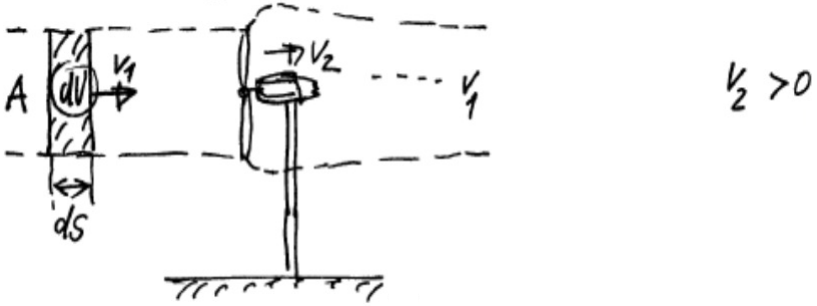
\includegraphics[width=0.95\columnwidth, align=c]{images/WEK_Leistungs-und_Drehzahlregelung.png}

$
\boxed{
P_{\text{max}} = \frac{dW}{dt} = \frac{A \cdot \rho_{\text{Luft}}}{2} \cdot v_1^3
}
\quad
\boxed{
P_W = c_P \cdot \frac{A \cdot \rho_{\text{Luft}}}{2} \cdot v_1^3
}
$ \quad Achtung! $v_1$ ist hoch 3!


\renewcommand{\arraystretch}{1.2}
\begin{tabular}{@{} l p{8cm} l @{}}
    $[P_{\text{max}}]$ & Theoretische Windleistung \dotfill & $W$ \\
    $[P_W]$            & Effektiv nutzbare praktische Windleistung \dotfill & $W$ \\
    $[c_P]$            & Leistungsbeiwert, $c_P = 0.4 ... 0.5$ \dotfill & $-$ \\
    $[A]$              & Rotorfläche (projizierte Fläche senkrecht zur Strömung) \dotfill & $m^2$ \\
    $[\rho_{\text{Luft}}]$ & Dichte Luft, $\approx 1{,}29 \, \frac{kg}{m^3}$ \dotfill & $\frac{kg}{m^3}$ \\
    $[v_1]$            & Anströmgeschwindigkeit des Windes \dotfill & $\frac{m}{s}$ \\
\end{tabular}



\section{Windenergiekonverter (WEK)}
\subsection{Netzkopplung}

DU = Direktumrichter, ZKU = Zwischenkreis-Umrichter\\

\subsubsection{Direkte Netzkopplung mit ASM}
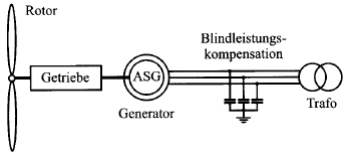
\includegraphics[width=0.6\columnwidth]{images/Direkte Netzkopplung mit ASM.png}

\subsubsection{Direkte Netzkopplung mit SM}
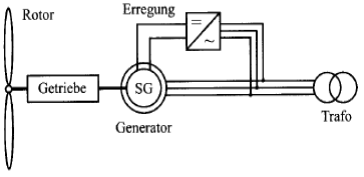
\includegraphics[width=0.6\columnwidth]{images/Direkte Netzkopplung mit SM.png}

\subsubsection{Direkte Netzkopplung mit ASM und DU im Läufer}
\includegraphics[width=0.6\columnwidth]{images/Direkte Netzkopplung mit ASM und Direktumrichter im Läufer.png}

\subsubsection{Direkte Netzkopplung mit SM über Gleichstromzwischenkreis}
\begin{itemize}
    \item variable Drehzahl
\end{itemize}

\vspace{0.1cm}

\includegraphics[width=0.6\columnwidth]{images/Direkte Netzkopplung mit SM über einen Gleichstromzwischenkreis, variable Drehzahl.png}

\subsubsection{Direkte Netzkopplung mit ASM und ZKU im Läufer}

\begin{itemize}
    \item übersynchrone Strorichter-Kaskade
    \item variable Drehzahl
\end{itemize}

\vspace{0.1cm}

\includegraphics[width=0.6\columnwidth]{images/Direkte Netzkopplung mit ASM und Zwischenkreis-umrichter im Läufer.png}















